\documentclass[aspectratio=169]{beamer}
%\documentclass{beamer}
%%%CHOOSE ASPECT RATIO ABOVE%%%

\usetheme{LU-spfaff}

\usepackage[utf8]{inputenc}
\usepackage[british]{babel}

\usepackage{url}
\usepackage{amssymb}


\usepackage{url}            % Nice URLs with line breaks
% \usepackage{xr}             % Cross-referencing -- for references etc
\usepackage{amsfonts}       % For eg. natural numbers
% \usepackage{amsthm}         % For thm, lemma, def
% \usepackage{amsmath}
% \usepackage{enumitem}       % For enumeration with roman numbers
\usepackage{mathrsfs}       % For (very) curly \mathscr
\usepackage{algorithm}      % For algorithms
\usepackage{algpseudocode}  % For algorithms
% \usepackage{scrextend}      % addmargin command
% \usepackage{subcaption}     % subfigures
% \usepackage{amssymb}        % for NAND symbol ($\barwedge$)
% \usepackage{textcomp}       % for trademark symbols
\usepackage{booktabs}       % for nice tables
% \usepackage{siunitx}        % round in tables

\title[XZDDF Bootstrapping]{XZDDF Bootstrapping}

\titlecolor{LUGreen} % Choose between LUPink, LULBlue, LUIvory, LUGreen
\titleimage{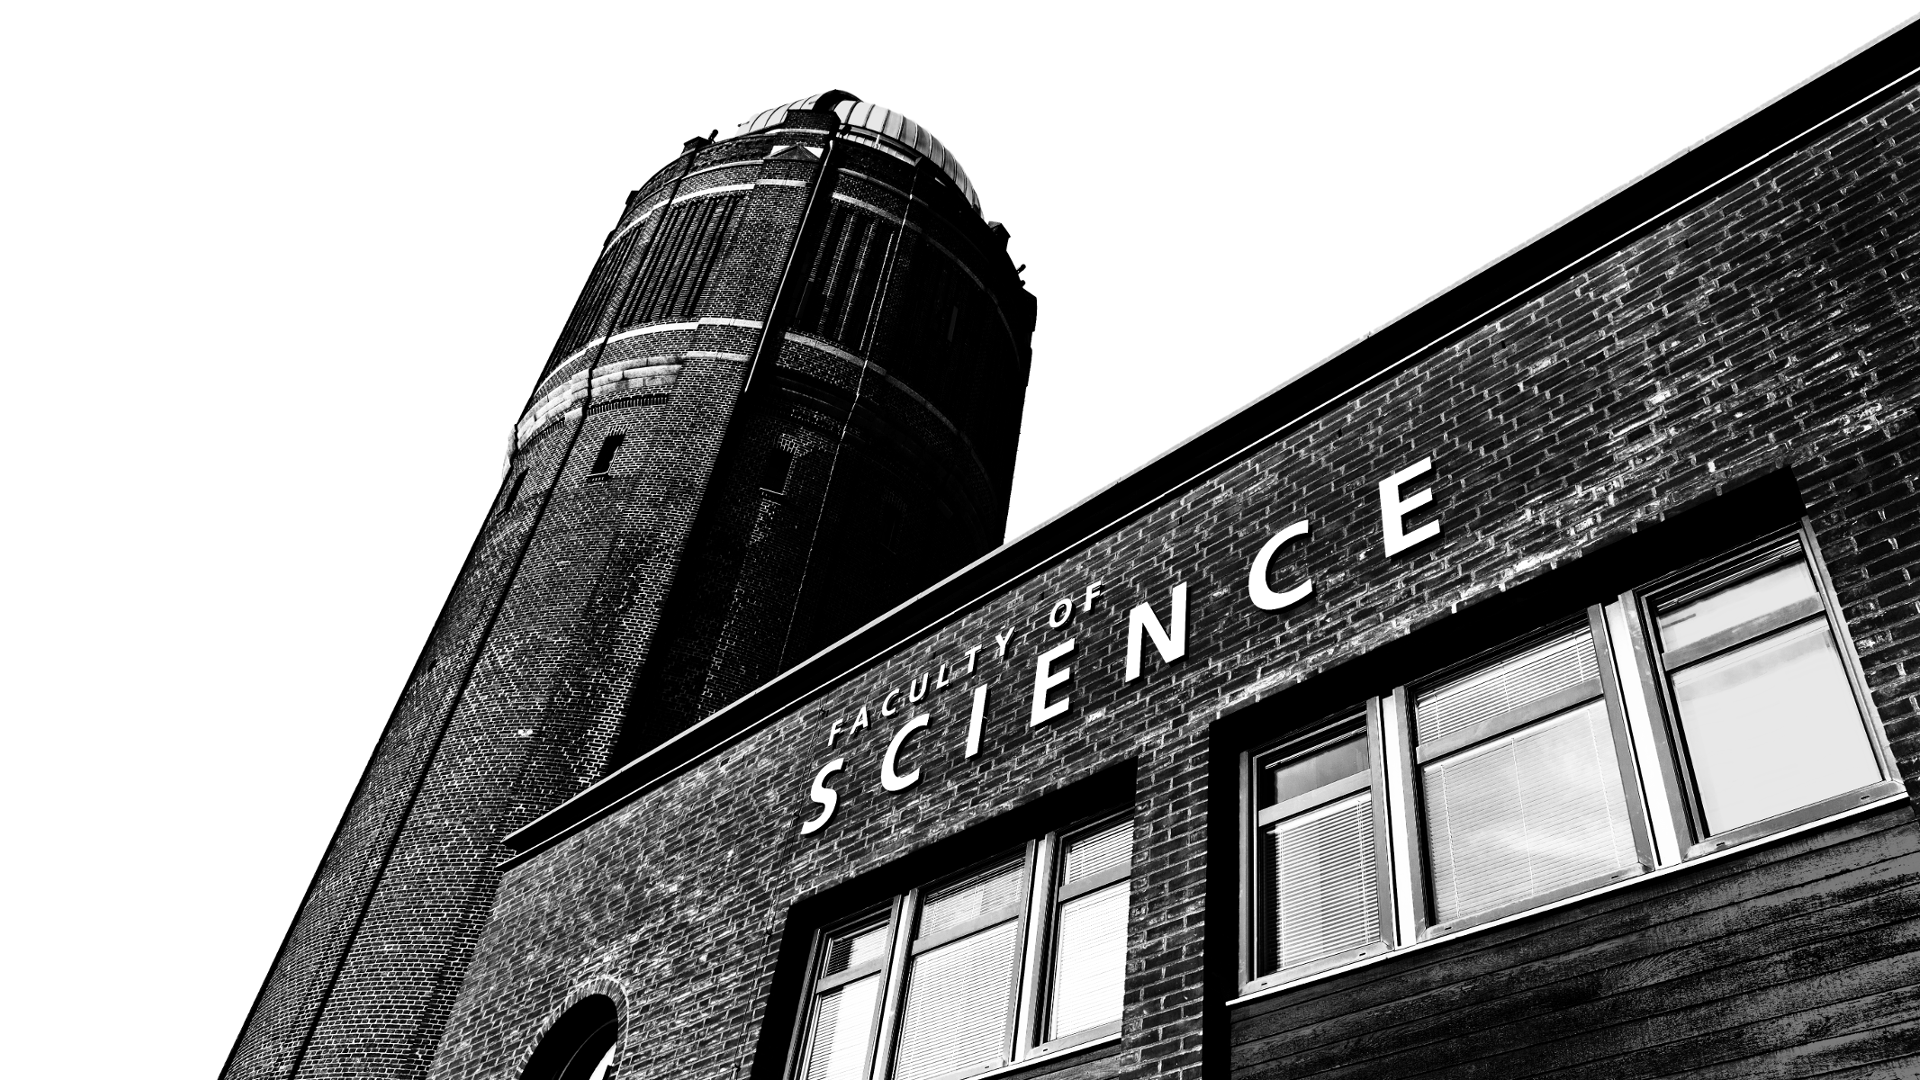
\includegraphics[scale=.5]{data/astro.png}}
% \titleimage{
\includegraphics[scale=.6]{data/lumainb.jpg}}
% \titleimage{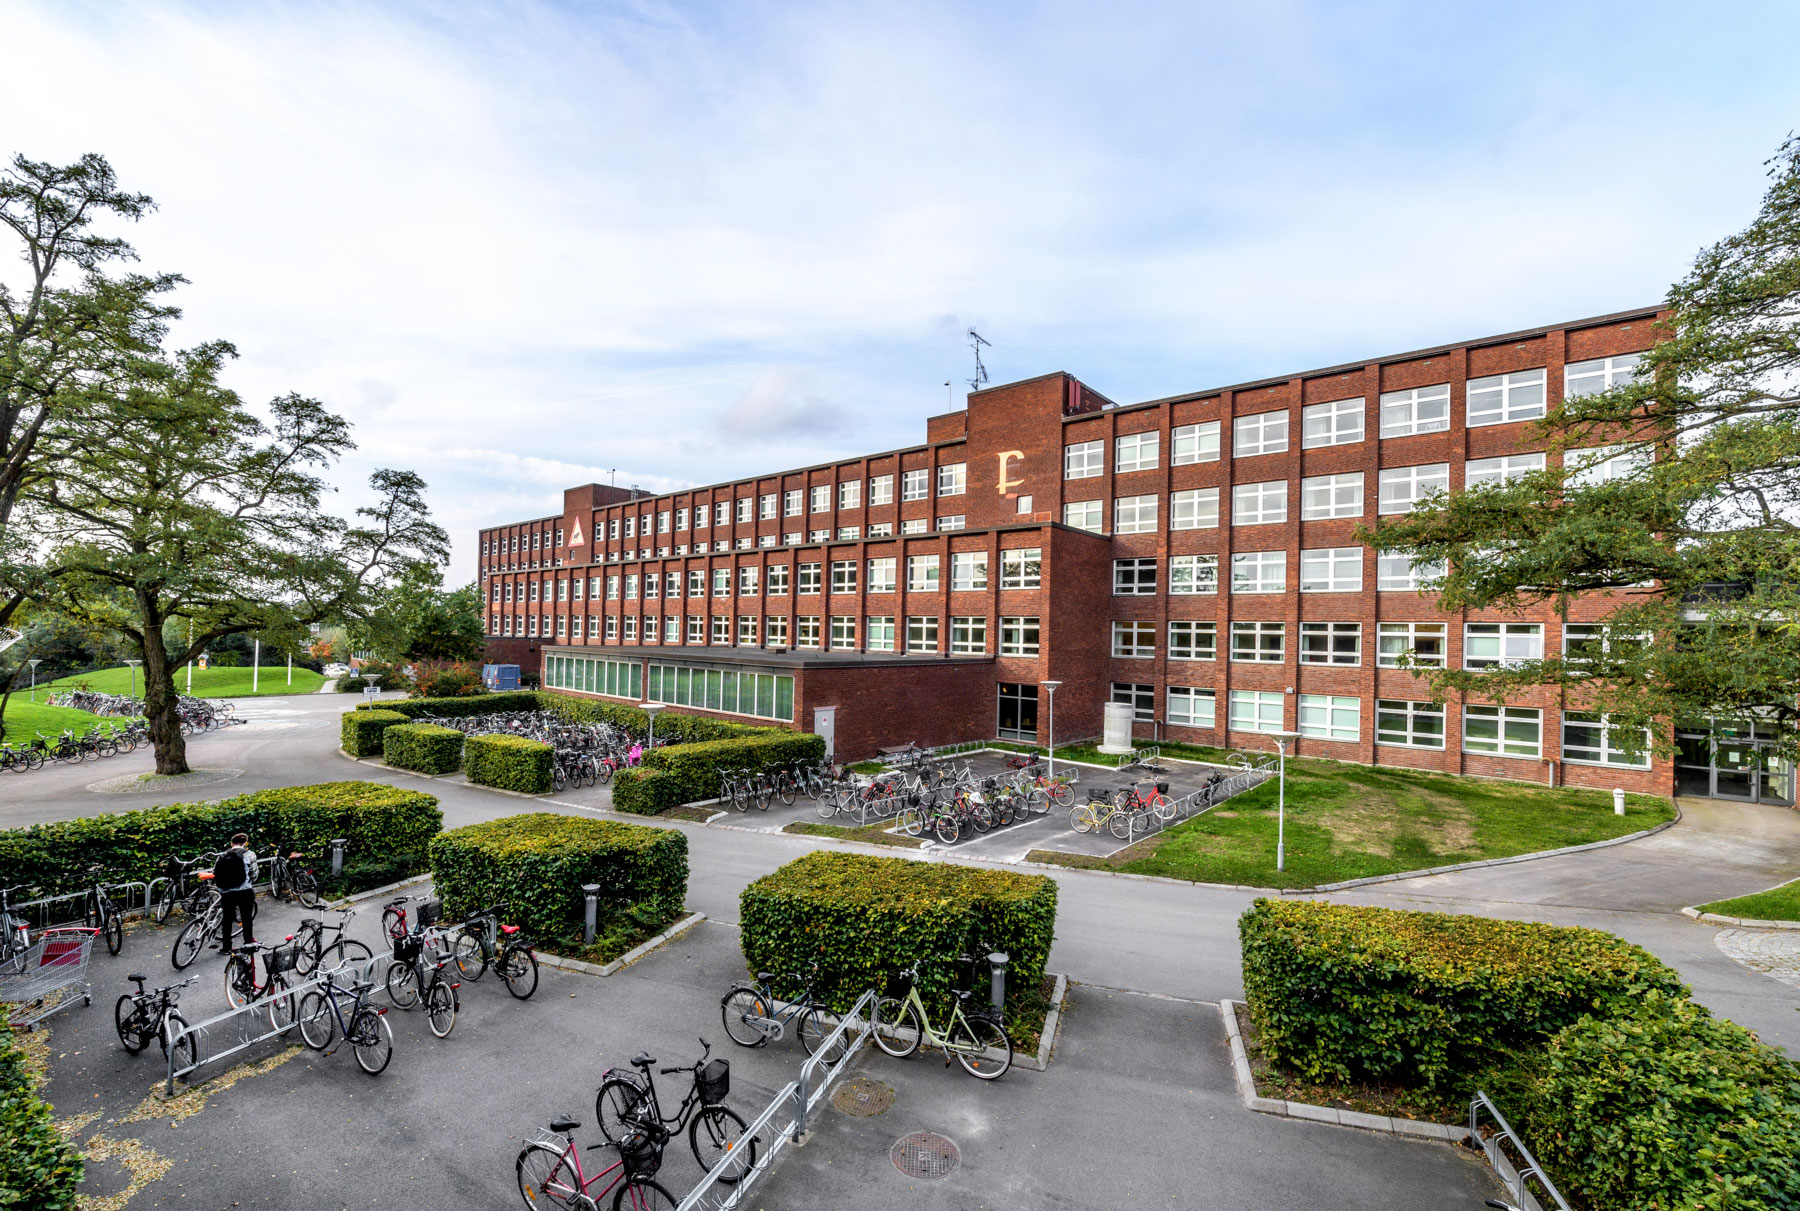
\includegraphics[scale=.25]{data/LTH_scampus_Matematikhuset_2_.jpg}}
\author{Simon Ljungbeck}
\subtitle{A Master's Thesis by Simon Ljungbeck}
\date{\today}
\institute{Lund University\\Department of Electrical and Information Technology}


\begin{document}

\titleframe
%-----
% Hello and welcome to the presentation of my master's thesis
%-----


%%%%%%%% Intro %%%%%%%%
\section{Introduction}

\begin{frame}{Project Description}
    \begin{itemize}
        \item Study Fully Homomorphic Encryption (FHE)
        \begin{itemize}
            \item How does it work?
            \item What are the main problems?
        \end{itemize}
    \end{itemize}
    \begin{itemize}
        \item Investigate XZDDF\footnote[frame]{\label{xzddf_paper} \url{https://eprint.iacr.org/2023/1564}} bootstrapping
    \end{itemize}
    \begin{itemize}
        \item Implement XZDDF$^1$ bootstrapping
    \end{itemize}
    % The authors did not publish their implementation (yet)
\end{frame}
%-----
% This project has mainly consisted of three parts. The first part was about studying FHE to understand how it works and to investigate why it is not used more in practice today. The second part was about investigating XZDDF bootstrapping, which is a new algorithm, published this year, for making FHE more efficient. The last part of the project was about implementing this new algorithm.
%-----



\begin{frame}{Outline}
    \begin{itemize}
        \item Introduction to FHE
    \end{itemize}
        \begin{itemize}
        \item XZDDF bootstrapping
    \end{itemize}
        \begin{itemize}
        \item Modification of XZDDF bootstrapping
    \end{itemize}
        \begin{itemize}
        \item Benchmark tests of XZDDF implementation
    \end{itemize}
\end{frame}
%-----
% The outline of this presentation looks like this. First, I will give a short introduction about what FHE is and how it works. Then I will explain how the new XZDDF algorithm works. After that, I will explain a modification of the algorithm I had to do because I found an error in the original algorithm. Finally, I will present the results of some efficiency tests I did on the implementation.
% The presentation will take about 25 minutes, and then there will be time for some questions, but, also, feel free to ask any question you have during the presentation as well.
%-----



%%%%%%%% FHE %%%%%%%%

\section{Fully Homomorphic Encryption}

\begin{frame}{\\~\\~\\~\\~\\~\\~\\ \huge \text{\;\;\;\;\;\;\;\;\;\;} Fully Homomorphic \\ \text{\;\;\;\;\;\;\;\;\;\;\;\;\;\;\;\;\;}  Encryption}
\end{frame}

\section{Fully Homomorphic Encryption}

\begin{frame}{What is Fully Homomorphic Encryption (FHE)?}
    % \begin{itemize}
    %     \item Let $\mathcal{E} = (\operatorname{KeyGen}, \operatorname{Enc}, \operatorname{Dec})$
    % \end{itemize}

    \begin{itemize}
        \item Let $c_1= \operatorname{Enc}(m_1)$ and $c_2= \operatorname{Enc}(m_2)$ be two ciphertexts
    \end{itemize}

    \begin{itemize}
        \item Assume we want to compute $c_3 = \operatorname{Enc}(m_1 + m_2)$
        \begin{itemize}
            \item Normally: $c_3 = \operatorname{Enc}(\operatorname{Dec}(c_1) + \operatorname{Dec}(c_2))$
            \item FHE: $c_3 = c_1 + c_2$
        \end{itemize}
    \end{itemize}

    \begin{itemize}
        \item FHE: \; $\operatorname{Enc}(f(m_1, \dots, m_t)) = f(\operatorname{Enc}(m_1), \dots, \operatorname{Enc}(m_t))$
    \end{itemize}
\end{frame}
%-----
% So, what is FHE? Let us say we have two ciphertexts c1 and c2 that encrypt m1 and m2. Then if we want to compute a ciphertext c3 that encrypts m1+m2, we would normally need to first decrypt c1 and c2, then add the plaintext messages, and then encrypt the result again. However, if an FHE scheme is used, we can just add the ciphertexts together. And in fact, with FHE any function can be evaluated without decrypting first, which this equation shows.
%-----

\begin{frame}{Why FHE?}
    \begin{itemize}
        \item Keep privacy when third parties do computations on data
        \begin{itemize}
            \item Cloud services
            \item Fog computing
        \end{itemize}
    \end{itemize}

    % \begin{itemize}
    %     \item Example: training an ML model on a supercomputer with sensitive data such as medical records or bank credentials
    % \end{itemize}

    \begin{itemize}
        \item Ex: training an ML model with sensitive data
    \end{itemize}

    \begin{itemize}
        \item Today's problem: FHE too inefficient
    \end{itemize}
\end{frame}
%-----
% This is not only a very cool property of an encryption scheme, but it also has several practical applications. One is for keeping privacy when third parties do computations on data. Since there is no need to decrypt the ciphertexts, one can do computations without knowing the data. For example, one can train a machine learning model in the cloud without revealing the training data. Although this sounds very appealing, FHE is not very much used in practice yet, and the main reason for this is that the existing algorithms are too slow.
%-----



% \begin{frame}{Some Notations}    
%     \begin{itemize}
%         \item $\mathcal{R} := \mathbb{Z}[X] / (X^N + 1)$, where $N := 2^k$ for some $k \in \mathbb{Z}^+$
%     \end{itemize}

%     \begin{itemize}
%         \item $\mathcal{R}_Q := \mathcal{R} / Q\mathcal{R} = \mathbb{Z}_Q[X] / (X^N + 1)$, where $\mathbb{Z}_Q := \mathbb{Z} / Q \mathbb{Z}$
%     \end{itemize}
% \end{frame}
%-----
% Now, I will explain FHE in more detail. First, I would like to introduce some notations that will be used in the rest of the presentation. R will be a polynomial ring over the integers modulo the polynomial X to the power of N plus one. If the integers are under modulo Q, we will denote the ring R_Q.
%-----


\begin{frame}{Noise-based FHE}
    \begin{itemize}
        \item FHE ciphertexts usually contain some noise 
    \end{itemize}
    
    \begin{itemize}
        \item Learning With Errors ($\operatorname{LWE}$): 
        \begin{itemize}
            \item $\operatorname{Enc}: \;\; \mathbb{Z}_q \ni m \mapsto \operatorname{LWE}_q (m) := (\mathbf{a}, b = \langle \mathbf{a}, \mathbf{s} \rangle + m + e \mod q) \in \mathbb{Z}_q^n \times \mathbb{Z}_q$ 
            \item $\operatorname{Dec}: \;\; c = (\mathbf{a}, b) \mapsto b - \langle \mathbf{a}, \mathbf{s} \rangle = m + e \approx m$
        \end{itemize}
    \end{itemize}

    % \begin{itemize}
    %     \item Ring Learning With Errors ($\operatorname{RLWE}$): 
    %     \begin{itemize}
    %         \item $ \operatorname{Enc}: \;\; \mathcal{R}_Q \ni m \mapsto \operatorname{RLWE}_Q (m) := (a, b = a \cdot s + m + e) \in \mathcal{R}_Q \times \mathcal{R}_Q$ 
    %         \item $\operatorname{Dec}: \;\; c = (a, b) \mapsto b  - a \cdot s = m + e \approx m$
    %     \end{itemize}
    % \end{itemize}
\end{frame}
%-----
% Most FHE schemes today are based on the LWE problem, or its ring version. An LWE encryption is a tuple of a vector a of integers modulo q, and an integer b, which is equal to the scalar product of a and the secret key s plus the message m plus some noise e. The important thing to note here is that the ciphertext contains the noise e. If knowing s, one can easily decrypt like this. There is also a corresponding problem in the ring R_Q, instead of the integers modulo q, which looks like this. As you can see, the notation is very similar.
%-----

\begin{frame}{The noise grows...}
    \begin{itemize}
        \item Homomorphic property of $\operatorname{LWE}$:
        %\begin{itemize}
            %\item $c_1 + c_2 = (\mathbf{a}_1, b_1) + (\mathbf{a}_2, b_2) = (\mathbf{a}_1 + \mathbf{a}_2, b_1 + b_2 = \langle \mathbf{a}_1, \mathbf{s} \rangle + \langle \mathbf{a}_2, \mathbf{s} \rangle + )$
            %\item
        %\end{itemize}
    \begin{align*}
                c_1 + c_2 &= (\mathbf{a}_1, b_1) + (\mathbf{a}_2, b_2) \\
                &= (\mathbf{a}_1 + \mathbf{a}_2, \langle \mathbf{a}_1, \mathbf{s} \rangle + \langle \mathbf{a}_2, \mathbf{s} \rangle + m_1 + m_2 + e_1 + e_2 ) \\
                &= (\mathbf{a}_1 + \mathbf{a}_2, \langle \mathbf{a}_1 + \mathbf{a}_2, \mathbf{s} \rangle + (m_1 + m_2) + (e_1 + e_2))
            \end{align*}
    \end{itemize}

    \begin{figure}
        \centering
        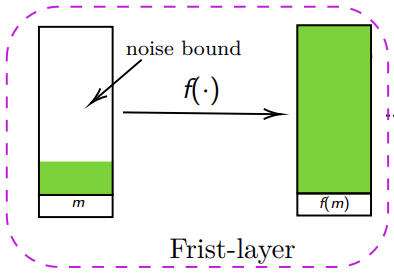
\includegraphics[scale=0.3]{data/noise.png}
        \caption{From Xiang et al.\footnote[frame]{\label{xzddf_slides} \url{https://iacr.org/cryptodb//data/paper.php?pubkey=33119}}}
        \label{fig:noise}
    \end{figure}
\end{frame}
%-----
% Here is an example how one can do addition homomorphically when using LWE encryption. One just add the elements of the tuple together. As can be seen, the noise is added together. In general, when the size of the noise increases when performing homomorphic operations, and at some point, the noise needs to be reduced to avoid decryption failure. This is what this figure is trying to illustrate.
%-----



\begin{frame}{Why is FHE slow?}

    \begin{itemize}
        \item Bootstrapping:
    \end{itemize}

    \begin{figure}
        \centering
        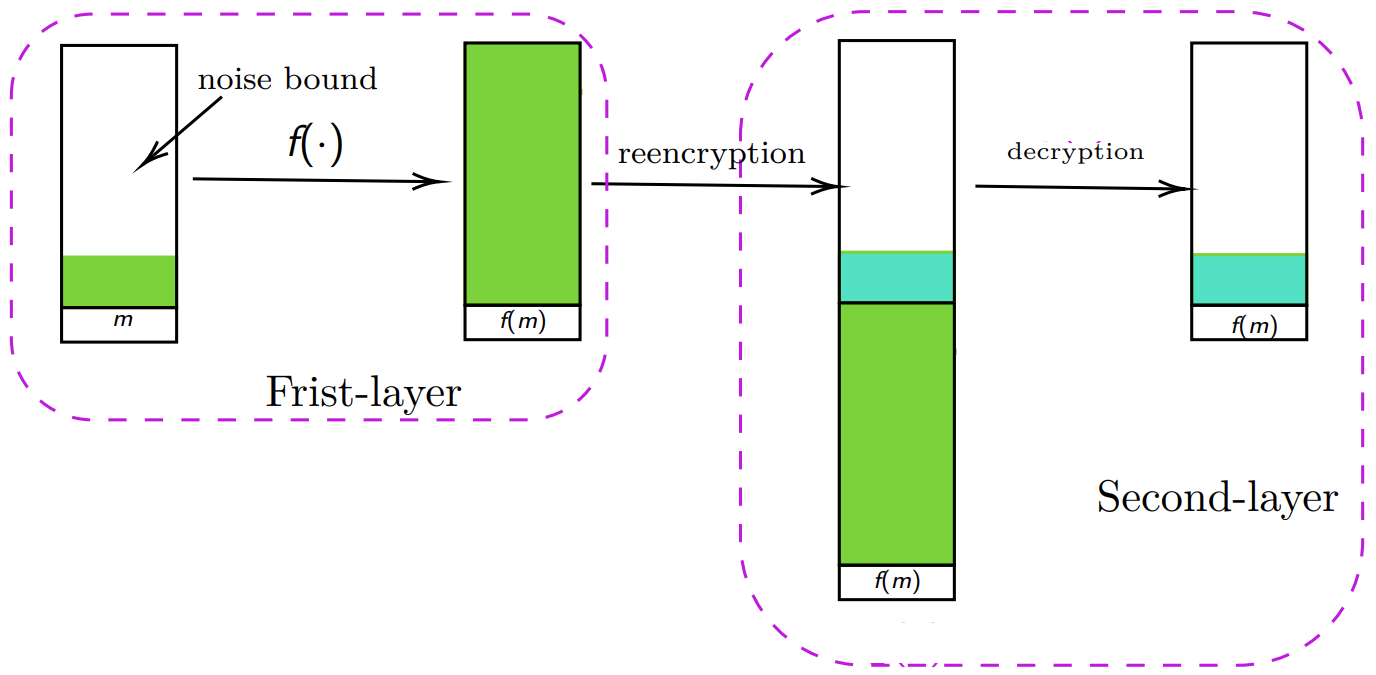
\includegraphics[scale=0.2]{data/bootstrap.png}
%        \caption{From Xiang et al.\footnote[frame]{\label{xzddf_slides} \url{https://iacr.org/cryptodb//data/paper.php?pubkey=33119}}}
        \label{fig:bootstrap}
    \end{figure}
    
    \begin{itemize}
        \item $\operatorname{LWE}: \;\; \operatorname{Dec}(c) = b - \langle \mathbf{a}, \mathbf{s} \rangle \mod q$ 
    \end{itemize}

\end{frame}
%-----
% There is a very elegant way of reducing the noise, and it can be illustraded like this. Firstly, one encrypts the ciphertext to a second layer, and then, since the scheme is fully homomorphic, one just evaluate its decryption function to remove the first layer and get a single-layered ciphertext again. Now, we can explain why FHE is so slow, because it is hard to do modulo computations homomorphically, which is needed to decrypt.
%-----



%%%%%%%% XZDDF %%%%%%%%
\section{XZDDF Bootstrapping}


\begin{frame}{\\~\\~\\~\\~\\~\\~\\~\\ \huge \text{\;\;\;\;\;\;\;} XZDDF Bootstrapping}
\end{frame}

\begin{frame}{XZDDF Bootstrapping}
    \begin{itemize}
        \item Assume first-layer: \;\; $(\mathbf{a}, b=\sum_{i=0}^{n-1}a_is_i - \operatorname{noised}(m)) \in \mathbb{Z}_q^n \times \mathbb{Z}_q$
        \begin{itemize}
            \item $\implies$ applicable with Regev, BGV, CKKS
            \item $\implies \operatorname{noised}(m) = \sum_{i=0}^{n-1}a_is_i -b \operatorname{\;\;mod} q$
        \end{itemize}        
    \end{itemize}

    \begin{itemize}
        \item $\mathcal{R}_Q := \mathbb{Z}_Q[X] / (X^N + 1)$ where $ N = 2^k \;\;\;\;\; \implies X^{2N} \equiv 1$ %\operatorname{ord}_{\mathcal{R}_Q}(X)=N$
    \end{itemize}
    
    \begin{itemize}
        \item Assume $q = 2N \implies X^{\operatorname{noised}(m)} = X^{\sum_{i=0}^{n-1}a_is_i -b \operatorname{\;\;mod} q} = X^{\sum_{i=0}^{n-1}a_is_i - b}$
        \begin{itemize}
            \item Let $r(X) = \sum_{i=0}^{q-1} iX^{-i} \implies \operatorname{noised}(m) = \operatorname{coeff}_0 \left(r(X) \cdot X^{\sum_{i=0}^{n-1}a_is_i - b}\right)$
        \end{itemize}
    \end{itemize}

    \begin{itemize}
        \item If $q|2N$ instead:
        \begin{itemize}
            \item $\left(X^{\frac{2N}{q}}\right)^q \equiv 1$
            \item $\operatorname{noised}(m) = \operatorname{coeff}_0 \left(r(X^{\frac{2N}{q}}) \cdot X^{-\frac{2N}{q}b} X^{\frac{2N}{q}\sum_{i=0}^{n-1}a_is_i}\right)$
        \end{itemize}
    \end{itemize}
\end{frame}
%-----
% So that was the introduction of FHE. Now, we will move over to XZDDF bootstrapping. This is an algorithm that is designed to do the modulo computations more efficiently. 
%-----


\begin{frame}{\\~\\~\\~\\~\\~\\~\\~\\ \huge \text{\;\;\;\;} More XZDDF Bootstrapping}
\end{frame}

\begin{frame}{XZDDF Bootstrapping}
    \begin{itemize}
        \item Assume $c_i(X) $ encrypts $X^{s_i}$ under $f(X) $
        % \item Assume $c_i(X) \in \mathcal{R}_Q$ encrypts $X^{s_i}$ under $f(X) \in \mathcal{R}_Q$
    \end{itemize}

    \begin{itemize}
        \item Automorphism: \; $c_i(X^{a_i})$ encrypts $X^{a_i s_i}$ under $f(X^{a_i}) $
        % \item Automorphism: \; $c_i(X^{a_i}) \in \mathcal{R}_Q $ encrypts $X^{a_i s_i}$ under $f(X) \in \mathcal{R}_Q$
        % \begin{itemize}
            % \item Problem 1: might have $2|a_i \implies a_i$ and $2N$ not coprime %\operatorname{gcd}(a_i, 2N) \neq 1$
            % \item Problem 2: want key $f(X)$, not $f(X^{a_i}) $
        % \end{itemize}
    \end{itemize}


    \begin{itemize}
        \item Problem 1: might have $2|a_i \implies a_i$ and $2N$ not coprime %\operatorname{gcd}(a_i, 2N) \neq 1$
        \begin{itemize}
            \item Solution: $q|N$ instead of $q|2N $%\implies X^{\frac{2N}{q}a_is_i} = X^{(\frac{2N}{q}a_i+1)s_i-s_i} = X^{w_is_i}X^{-s_i}$
            \begin{align*}
                & \implies X^{\frac{2N}{q}a_is_i} = X^{(\frac{2N}{q}a_i+1)s_i-s_i} = X^{w_is_i}X^{-s_i}, \text{ where $w_i$ is odd} %\\
                % & \text{i.e. want } \operatorname{noised}(m) = \operatorname{coeff}_0 \left(r(X^{\frac{2N}{q}}) \cdot X^{-\frac{2N}{q}b} X^{\sum_{i=0}^{n-1}w_is_i} X^{-\sum_{i=0}^{n-1}s_i}\right)
            \end{align*}
        \end{itemize}
    \end{itemize}

    \begin{itemize}
        \item Problem 2: want key $f(X)$, not $f(X^{a_i}) $
        \begin{itemize}
            \item Solution: use NTRU encryption...
        \end{itemize}
    \end{itemize}

\end{frame}


\begin{frame}{NTRU Encryption}
    \begin{itemize}
        \item Define
            \begin{equation*}
              (\tau, \Delta) :=
                \begin{cases}
                  \left(1, \left\lfloor \frac{Q}{t} \right\rceil \right), & \text{if $\operatorname{noised}(m) = e + \left \lfloor \frac{q}{t} \right \rceil \cdot m$} \\
                  (t,1), & \text{if $\operatorname{noised}(m) = t \cdot e + m$}\\
                  (1,1), & \text{if $\operatorname{noised}(m) = e + m$}.
                \end{cases}       
            \end{equation*}
    \end{itemize}
    
    \begin{itemize}
        \item Scalar NTRU encryption: \; $\mathrm{NTRU}_{Q, f, \tau, \Delta}(u) := \tau \cdot g/f + \Delta \cdot u/f \in \mathcal{R}_Q$
    \end{itemize}
    
    \begin{itemize}
        \item Vector NTRU encryption: \; $\mathrm{NTRU}'_{Q, f, \tau}(v) := (\tau \cdot g_0/f + B^0\cdot v, \ldots, \tau \cdot g_{d-1}/f + B^{d-1}\cdot v) \in \mathcal{R}_Q^d$
    \end{itemize}
\end{frame}

\begin{frame}{Homomorphic Multiplication for NTRU}
    \begin{itemize}
        \item $\operatorname{BitDecom}_B(a) := (a_0, \ldots, a_{d-1}) \in \mathcal{R}_B^d,$ where $a = \sum_{i=0}^{d-1}a_i\cdot B^i$
    \end{itemize}
    \begin{itemize}
        \item $c \odot \mathbf{c}' := \langle \operatorname{BitDecom}_B(c), \mathbf{c}' \rangle = \sum_{i=0}^{d-1}c_ic_i'=\tau \cdot \sum_{i=0}^{d-1} c_i g_i / f + cv \in \mathcal{R}_Q$
    \end{itemize}
    \begin{itemize}
        \item \textbf{Lemma 4.1} (Homomorphic multiplication)\textbf{.} Assume that $c = \mathrm{NTRU}_{Q, f, \tau, \Delta}(u)$ and $\mathbf{c}' = \mathrm{NTRU}'_{Q, f, \tau}(v) $. Then $\hat{c} = c \odot \mathbf{c}'$ is a scalar NTRU ciphertext of $uv$.
    \end{itemize}
\end{frame}

\begin{frame}{NTRU Key Switching}
    \begin{itemize}
        \item $\mathbf{ksk}_{f_1,f_2} := (\tau \cdot g_0/f_2 + B^0 \cdot f_1/f_2, \ldots, \tau \cdot g_{d-1}/f_2 + B^{d-1} \cdot f_1/f_2)$
    \end{itemize}

    \begin{itemize}
        \item \textbf{Lemma 4.2} (NTRU key switching)\textbf{.} The product $c \odot \mathbf{ksk}_{f_1,f_2}$ is a scalar NTRU encryption of the same message as $c$ but under the new private key $f_2 \in \mathcal{R}_Q$.
        % \begin{itemize}
        \\ $\implies$ Problem 2 solved
        % \end{itemize}
    \end{itemize}    
\end{frame}

\begin{frame}{Generating the Blind Rotation Key}
    \begin{figure}
        \centering
        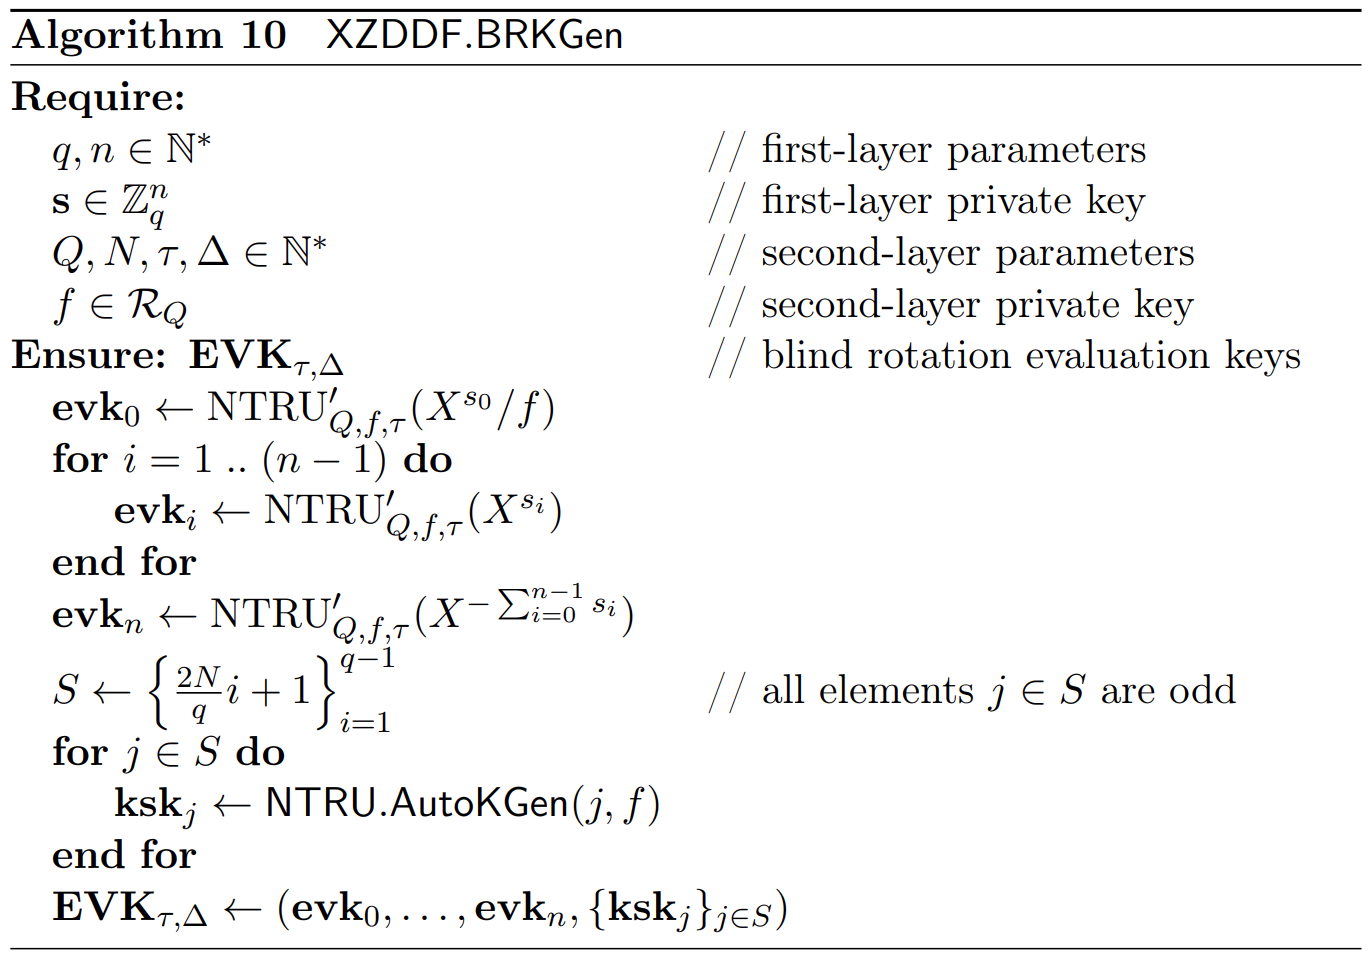
\includegraphics[scale=0.2]{data/brkgen.png}
        \label{fig:brkgen}
    \end{figure}
\end{frame}

\begin{frame}{Performing the Blind Rotation}
    \begin{figure}
        \centering
        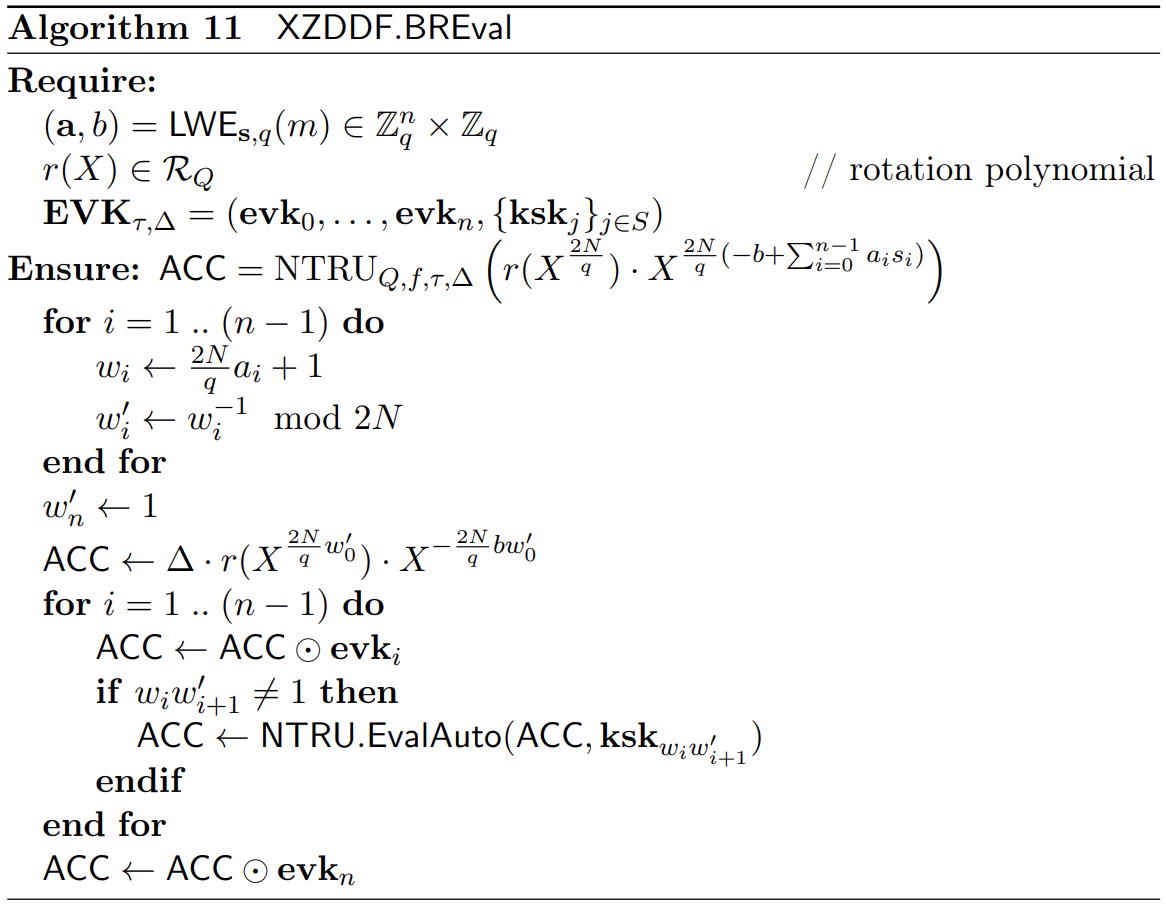
\includegraphics[scale=0.21]{data/breval.png}
        \label{fig:breval}
    \end{figure}
\end{frame}

\begin{frame}{Extraction}
    \begin{itemize}
        \item After the blind rotation, we get a ciphertext 
            $$c = \mathrm{NTRU}_{Q, f, \tau, \Delta}\left(r(X^{\frac{2N}{q}}) \cdot X^{\frac{2N}{q} (-b  + \sum_{i=0}^{n-1}a_is_i)}\right)$$
    \end{itemize}
    \begin{itemize}
        \item Define
        \begin{align*}
            &\mathbf{f} = (f_0, \ldots, f_{N-1}) \in \mathbb{Z}_Q^N \\
            &\hat{\mathbf{c}} = (c_0, -c_{N-1}, \ldots, -c_1) \in \mathbb{Z}_Q^N
        \end{align*}
    \end{itemize}
    % \begin{itemize}
    %     \item Then $$0 = \langle \hat{\mathbf{c}}, \mathbf{f} \rangle - (\tau \cdot g_0 + \Delta \cdot \operatorname{noised}(m)) \in \mathbb{Z}_Q$$
    % \end{itemize}
    \begin{itemize}
        \item Then $$(\hat{\mathbf{c}}, 0) \in \mathbb{Z}_Q^N \times \mathbb{Z}_Q = \operatorname{LWE}_{Q,\mathbf{f}}(m)$$
    \end{itemize}
\end{frame}

\section{Modification of XZDDF}

\begin{frame}{\\~\\~\\~\\~\\~\\~\\~\\ \huge \text{\;\;\;\;\;\;\;\;} Modification of XZDDF}
\end{frame}

\begin{frame}{The Problem...}
    \begin{itemize}
        \item Want to compute
        $$\operatorname{noised}(m) = \operatorname{coeff}_0 \left(r(X^{\frac{2N}{q}}) \cdot X^{\frac{2N}{q} (-b  + \sum_{i=0}^{n-1}a_is_i)}\right),$$
        where $r(X^{\frac{2N}{q}}) = \sum_{i=0}^{q-1} iX^{- \frac{2N}{q} \cdot i}$
    \end{itemize}
    \begin{itemize}
        \item But in $\mathcal{R}_Q = \mathbb{Z}_Q[X] / (X^N + 1)$ we have that
        \begin{equation*}
          X^{-i} =
            \begin{cases}
              1, & \text{if $i=0$} \\
              -X^{N-i}, & \text{if $1 \leq i \leq N$}\\
              X^{2N-i}, & \text{if $N+1 \leq i \leq 2N-1$}.
            \end{cases}       
        \end{equation*}
    \end{itemize}
\end{frame}
%-----
% N=2: X^-0 = 1, X^-1=-X, X^-2=-1, X^-3=X
%-----


\begin{frame}{The Problem...}
    \begin{itemize}
        \item If for example $q=2N$, we get
        \begin{align*}
            r(X) &= \sum_{i=0}^{q-1} iX^{-i} \\
            &= -1 \cdot X^{N-1} -2 \cdot X^{N-2} - \dots - N + \\
            & \;\;\;\; + (N+1) \cdot X^{N-1} + (N+2) \cdot X^{N-2} + \dots + (2N-1) \cdot X \\
            & = -N + N \cdot X + N \cdot X^2 + \dots + N \cdot X^{N-1}.
        \end{align*}
    \end{itemize}
    \begin{itemize}
        \item Same problem for any $q|N$ %-- half of the terms still wraps around
    \end{itemize}
\end{frame}

\begin{frame}{A Suggestion of Solution}
    \begin{itemize}
        \item Assume
        \begin{cases}
            \text{Boolean operations} \\
            \text{Binary messages} \\
            \text{Regev-like first-layer encryption}
        \end{cases}
    \end{itemize}
    \begin{itemize}
        \item $\operatorname{LWE}^{\text{Regev}}_{q,\mathbf{s}}(m) = \left(\mathbf{a}, b = \langle \mathbf{a}, \mathbf{s} \rangle + m \cdot \frac{q}{t} + e\right) \in \mathbb{Z}_q^n \times \mathbb{Z}_q$
        \begin{itemize}
            \item We will use $t=4$
        \end{itemize}
    \end{itemize}
\end{frame}

\begin{frame}{A Suggestion of Solution}
    \begin{itemize}
        \item Let $\diamond$ denote a binary operation
    \end{itemize}
    \begin{itemize}
        \item Let $c_1 = (\mathbf{a}_1,b_1)$ and $c_2 = (\mathbf{a}_2,b_2)$
    \end{itemize}
    \begin{itemize}
        \item Start by computing $c = c_1 + c_2 = (\mathbf{a}_1 + \mathbf{a}_2, b_1 + b_2) =: (\mathbf{a},b)$
        \begin{equation*}
          \implies \operatorname{Dec}(c) =
            \begin{cases}
              0, & \text{if $(m_1, m_2) = (0,0)$} \\
              1, & \text{if $(m_1, m_2) = (0,1)$ or $(1,0)$}\\
              2, & \text{if $(m_1, m_2) = (1,1)$}
            \end{cases}
        \end{equation*}
    \end{itemize}
\end{frame}

\begin{frame}{A Suggestion of Solution}
    % \begin{itemize}
    %     \item Denote $\operatorname{noised}(m) := b - \langle \mathbf{a}, \mathbf{s} \rangle = m \cdot \frac{q}{t} + e$
    % \end{itemize}
    \begin{itemize}
        \item Define $t$ intervals
        $I_i = \left[ i \cdot \frac{q}{t} - \frac{q}{2t},  i \cdot \frac{q}{t} + \frac{q}{2t}\right) \subset \mathbb{Z}_q$ for $i=0,1,2,t-1$
        \begin{align*}
            I_0 &= \left[-\frac{q}{8}=\frac{7q}{8}, \frac{q}{8}\right), \\
            I_1 &= \left[\frac{q}{8}, \frac{3q}{8}\right), \\
            I_2 &= \left[\frac{3q}{8}, \frac{5q}{8}\right), \\
            I_3 &= \left[\frac{5q}{8}, \frac{7q}{8}\right).
        \end{align*}
    \end{itemize}
\end{frame}

\begin{frame}{A Suggestion of Solution}
    \begin{itemize}
        \item If for example $\diamond = \operatorname{OR}$, we now want a function $f_{\operatorname{OR}}$ that maps
        \begin{equation*}
          f_{\operatorname{OR}}: \;\; \left (X^{\frac{2N}{q}}\right)^{\operatorname{noised}(m)} \mapsto
            \begin{cases}
              0, & \text{if $\operatorname{noised}(m) \in I_0$} \\
              1, & \text{if $\operatorname{noised}(m) \in I_1$} \\
              1, & \text{if $\operatorname{noised}(m) \in I_2$} \\
              0, & \text{if $\operatorname{noised}(m) \in I_3$}.
            \end{cases}
        \end{equation*}
    \end{itemize}
\end{frame}

\begin{frame}{A Suggestion of Solution}
    \begin{itemize}
        \item If for example $\diamond = \operatorname{AND}$, we now want a function $f_{\operatorname{AND}}$ that maps
        \begin{equation*}
          f_{\operatorname{AND}}: \;\; \left (X^{\frac{2N}{q}}\right)^{\operatorname{noised}(m)} \mapsto
            \begin{cases}
              0, & \text{if $\operatorname{noised}(m) \in I_0$} \\
              0, & \text{if $\operatorname{noised}(m) \in I_1$} \\
              1, & \text{if $\operatorname{noised}(m) \in I_2$} \\
              1, & \text{if $\operatorname{noised}(m) \in I_3$}.
            \end{cases}
        \end{equation*}
    \end{itemize}
\end{frame}

\begin{frame}{A Suggestion of Solution}
    \begin{itemize}
        \item It turns out (see \texttt{OpenFHE}) that $[0,q)$ can always be split into two intervals
        \begin{align*}
            &I^0 = I_{k} \cup I_{(k+1 \text{ mod 4})}\\
            &I^1 = I_{(k+2 \text{ mod 4})} \cup I_{(k+3 \text{ mod 4})}
        \end{align*}
        \item Ex: \;\;
        % \begin{equation*}
            \begin{cases}
                $\operatorname{OR} \implies k=3$ \\
                $\operatorname{AND} \implies k=0$
            \end{cases}
        % \end{equation*}
    \end{itemize}
    \begin{itemize}
        \item Let $I^0 = [q_0,q_1)$ and $I^1 = [q_1,q_0)$
    \end{itemize}
\end{frame}

\begin{frame}{A Suggestion of Solution}
    \begin{itemize}
        \item Negacyclical property of $\mathcal{R}_Q$: \;\; $aX^i \equiv -aX^{i+N} \mod (X^N+1)$
    \end{itemize}
    \begin{itemize}
        \item Use
            \begin{align*}
            r(X^{\frac{2N}{q}}) = -1 & \cdot \left(X^{-\frac{2N}{q}}\right)^0 - 1 \cdot \left(X^{-\frac{2N}{q}}\right)^1 - \dots - 1 \cdot \left(X^{-\frac{2N}{q}}\right)^{\frac{q}{4}-1} + \\
            &+ 1 \cdot \left(X^{-\frac{2N}{q}}\right)^{\frac{q}{4}} + \dots + 1 \cdot \left(X^{-\frac{2N}{q}}\right)^{\frac{q}{2}-1}.
            \end{align*}
        \begin{align*}
            \implies 
            m':&=\operatorname{coeff}_0\left(r(X^{\frac{2N}{q}}) \cdot \left(X^{\frac{2N}{q}(\operatorname{noised}(m)+(\frac{q}{4}-q_1))}\right)\right) = \\
            &= \begin{cases}
              -1, & \text{if $\operatorname{noised}(m) \in [q_0, q_1) = I^0$} \\
              1, & \text{if $\operatorname{noised}(m) \in [q_1, q_0) = I^1$}.
            \end{cases}
        \end{align*}
    \end{itemize}
\end{frame}

\begin{frame}{A Suggestion of Solution}
    \begin{itemize}
        \item Now, we just want to map
        \begin{equation*}
            m' \mapsto
            \begin{cases}
              0, & \text{if $m' = -1$} \\
              1, & \text{if $m' = 1$}.
            \end{cases}
        \end{equation*}
    \end{itemize}
    \begin{itemize}
        \item $c' = \operatorname{LWE}_{Q,\mathbf{f}}(m') = (\mathbf{a}, b' = \langle \mathbf{a}, \mathbf{s} \rangle + \Delta \cdot m' + e)$
        \begin{itemize}
            \item Choose $\Delta = \frac{Q}{4} \cdot \frac{1}{2} = \frac{Q}{8}$
            \begin{equation*}
                \implies c' = \operatorname{LWE}_{Q,\mathbf{f}}(m') =
                \begin{cases}
                  (\mathbf{a}, b' = \langle \mathbf{a}, \mathbf{s} \rangle - \frac{Q}{8} + e), & \text{if $m' = -1$} \\
                  (\mathbf{a}, b' = \langle \mathbf{a}, \mathbf{s} \rangle + \frac{Q}{8} + e), & \text{if $m' = 1$}. \\
                \end{cases}
            \end{equation*}
        \end{itemize}
    \end{itemize}
\end{frame}

\begin{frame}{A Suggestion of Solution}
    \begin{itemize}
        \item Finally, add $Q/8$ to $b'$
        $$c = (\mathbf{a},b) = \left(\mathbf{a},b' + \frac{Q}{8}\right)$$
        \begin{align*}
            \implies c = \operatorname{LWE}_{Q,\mathbf{f}}(m') &=
            \begin{cases}
              (\mathbf{a}, b = \langle \mathbf{a}, \mathbf{s} \rangle + e), & \text{if $m' = -1$} \\
              (\mathbf{a}, b = \langle \mathbf{a}, \mathbf{s} \rangle + \frac{Q}{4} + e), & \text{if $m' = 1$},
            \end{cases} \\
            \implies m = \operatorname{Dec}(c) &=
            \begin{cases}
              0, & \text{if $m' = -1$} \\
              1, & \text{if $m' = 1$},
            \end{cases}
        \end{align*}
    \end{itemize}
\end{frame}


%%%%%%%% Benchmarking %%%%%%%%
\section{Benchmark Tests}

\begin{frame}{\\~\\~\\~\\~\\~\\~\\~\\ \huge \text{\;\;\;\;\;\;\;\;\;\;\;\;\;} Benchmark Tests}
\end{frame}


\begin{frame}{Implementation}
    \begin{itemize}
        \item Implemented XZDDF in \texttt{OpenFHE}
        \item See \url{https://github.com/SL2000s/masters_thesis_xzddf}
    \end{itemize}    
\end{frame}

\begin{frame}{Tests}
    \begin{table}[ht]
    \centering
    % \caption{Simple tests}
    \begin{tabular}{cl}
    \toprule
    \textbf{Test} & \textbf{Description} \\
    \midrule
    \text{S1:} & Generating a bootstrapping key. \\
    \text{S2:} & Performing a single bootstrapping. \\
    \text{S3:} & Performing an OR operation on two ciphertexts \(c_0\) and \(c_1\). \\
    \text{S4:} & Performing an AND operation on two ciphertexts \(c_0\) and \(c_1\). \\
    % \hline
    % \text{B1:} & Updating $c_1$ with the value of $f(c_0,c_1)$ 1 time. \\
    % \text{B2:} & Updating $c_1$ with the value of $f(c_0,c_1)$ 10 times. \\
    % \text{B3:} & Updating $c_1$ with the value of $f(c_0,c_1)$ 100 times. \\
    % \text{B4:} & Updating $c_1$ with the value of $f(c_0,c_1)$ 1000 times. \\
    \bottomrule
    \end{tabular}
    \label{tab:simple_tests}
    \end{table}    
\end{frame}

\begin{frame}{Results}
    \begin{table}[ht]
        \centering
        \begin{tabular}{lc|cccc}
        \toprule
        \textbf{Algorithm} & \textbf{Param.} & \textbf{S1} (ms)  & \textbf{S2} (ms) & \textbf{S3} (ms) & \textbf{S4} (ms) \\
        \midrule
        AP & STD128 & 10541 & 182 & 175 & 175 \\
        GINX & STD128 & 2583 & 153 & 145 & 145 \\
        LMKCDEY & STD128L & 2121 & 120 & 132 & 134 \\
        XZDDF & STD128 & 2438 & 174 & 184 & 185 \\
        XZDDF & P128T & 6386 & 214 & 216 & 216 \\
        XZDDF & P128G & 5820 & 194 & 195 & 195 \\
        AP & STD192 & 38489 & 651 & 662 & 645 \\
        GINX & STD192 & 8546 & 467 & 467 & 468 \\
        LMKCDEY & STD192 & 8833 & 493 & 512 & 435 \\
        XZDDF & STD192 & 8391 & 626 & 622 & 626 \\
        XZDDF & P192T & 11808 & 700 & 699 & 699 \\
        XZDDF & P192G & 9989 & 592 & 592 & 592 \\
        \bottomrule
        \end{tabular}
        \label{tab:efficiency_res}
    \end{table}
\end{frame}

% \begin{frame}{Results}
%     \begin{figure}
%         \centering
%         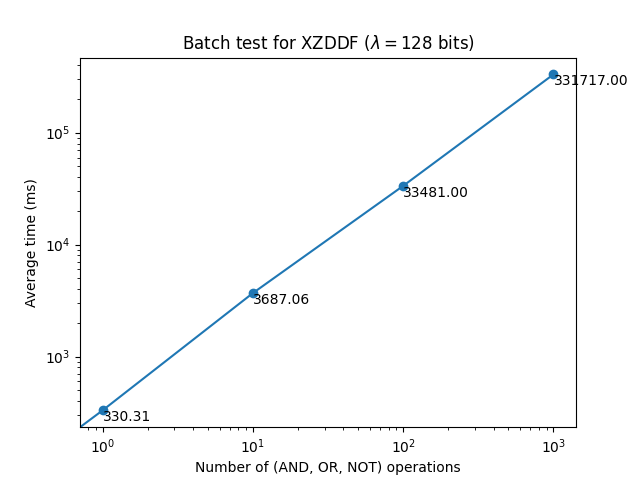
\includegraphics[scale=0.5]{data/XZDDF_STD128_batch.png}
%         \label{fig:batch_res}
%     \end{figure}
% \end{frame}

%%%%%%%% Conclusions %%%%%%%%
\section{Conclusions}

\begin{frame}{Conclusions}
    \begin{itemize}
        \item XZDDF implementation performs quite well at key generation
    \end{itemize}
    \begin{itemize}
        \item XZDDF implementation not as fast as it theoretically should
        \begin{itemize}
            \item LMKCDEY still seems to be faster
        \end{itemize}
    \end{itemize}
    \begin{itemize}
        \item Bootstrapping is the main bottleneck in all FHE algorithms
        % \begin{itemize}
        %     \item Execution time linear in the number of bootstrappings
        % \end{itemize}
    \end{itemize}
    \begin{itemize}
        \item New rotation polynomial works, but only for a special case
    \end{itemize}    
\end{frame}

\begin{frame}{Visions and Future Work}
    \begin{itemize}
        \item Find a rotation polynomial $r(X)$ for the general case?
    \end{itemize}    
    \begin{itemize}
        \item More efficient XZDDF implementation?
    \end{itemize}    
    \begin{itemize}
        \item FHE still needs to become more efficient
    \end{itemize}
    \begin{itemize}
        \item Bootstrapping 2010: 30 minutes
        \item Today: 100~ms
    \end{itemize}    
\end{frame}

\begin{frame}%{Thank You For Listening}
\begin{center}
\Huge Thank you for listening! \\~\\
\Large Questions?
% \\~\\ \small Acknowledgments: Qian Guo (supervisor), Thomas Johansson (examinor)
\end{center}
\\~\\~\\ \small Acknowledgments:
\begin{itemize}
\begin{itemize}
    \item Supervisor: Qian Guo
    \item Examiner: Thomas Johansson
\end{itemize}
\end{itemize}
\end{frame}



\end{document}